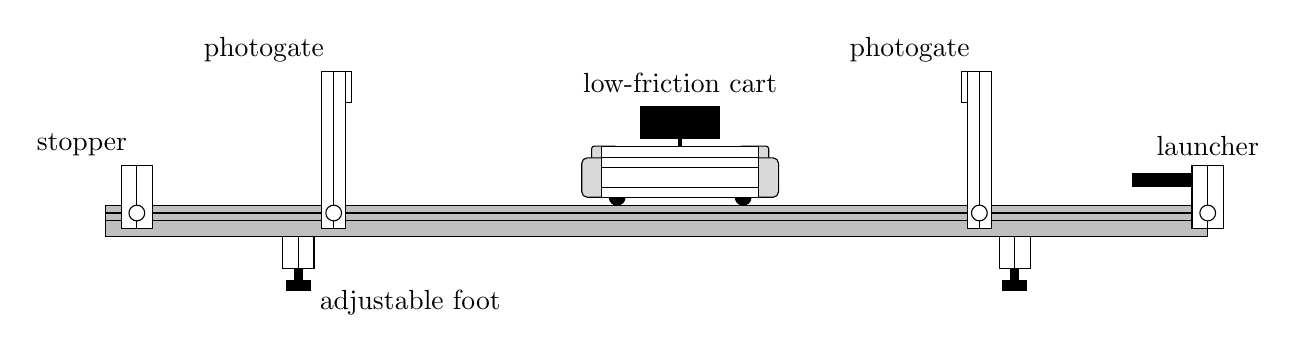
\begin{tikzpicture}
    \def\L{14}          % track length
    \def\t{0.2}         % track thickness
    \def\fx{2.25}       % foot distance from edge
    \def\fw{0.2}        % foot width
    \def\fh{0.4}        % foot height
    \def\sx{0.2}        % stopper distance from edge
    \def\sw{\fw}        % stopper width
    \def\sh{0.8}        % stopper height
    \def\soffset{0.1}   % stopper offset
    \def\pgx{2.75}      % photogate distance from edge
    \def\pgw{0.15}      % photogate width
    \def\pgh{2}         % photogate height
    \def\pgoffset{0.1}  % photogate offset
    \def\cw{2}          % cart width
    \def\ch{0.5}        % cart height
    \def\cx{0.45*\L}    % cart edge position
    \def\coffset{(2*\t+0.1)}   % cart offset from track
    % Draw the track bed
    \draw[fill=gray!50] (0,0) rectangle (\L,\t);
    \draw[fill=gray!50] (0,\t) rectangle (\L,{1.5*\t});
    \draw[fill=gray!50] (0,{1.5*\t}) rectangle (\L,{2*\t});
    % Draw the track feet
    \begin{scope}[shift={(\fx,-\fh)}]
        \draw[fill=white] (0,0) rectangle (\fw,\fh);
        \draw[fill=white] (\fw,0) rectangle ({2*\fw},\fh);
        \filldraw[black] (0.05,{-0.7*\fh}) rectangle ({2*\fw-0.05},{-0.4*\fh}) node[below right] {adjustable foot};
        \filldraw[black] ({0.75*\fw},{-0.4*\fh}) rectangle ({1.25*\fw},0);
    \end{scope}
    \begin{scope}[shift={({\L-\fx-2*\fw},-\fh)}]
        \draw[fill=white] (0,0) rectangle (\fw,\fh);
        \draw[fill=white] (\fw,0) rectangle ({2*\fw},\fh);
        \filldraw[black] (0.05,{-0.7*\fh}) rectangle ({2*\fw-0.05},{-0.4*\fh});
        \filldraw[black] ({0.75*\fw},{-0.4*\fh}) rectangle ({1.25*\fw},0);
    \end{scope}
    % Draw the stopper
    \draw[fill=white] (\sx,\soffset) rectangle ({\sx+\sw},{\soffset+\sh}) node[above left] {stopper};
    \draw[fill=white] ({\sx+\sw},\soffset) rectangle ({\sx+2*\sw},{\soffset+\sh});
    \draw[fill=white] ({\sx+\sw}, {3*\soffset}) circle (1mm);
    % Draw the cart and flag
    \begin{scope}[shift={(\cx,\coffset)}]
        \draw[fill=black] (0.2,0) circle (1mm);
        \draw[fill=black] ({\cw-0.2},0) circle (1mm);
        \draw[fill=gray!30, rounded corners=1] (-0.125,{\ch-0.15}) rectangle (0.2,{\ch+0.15});
        \draw[fill=gray!30, rounded corners=1] ({\cw-0.25},{\ch-0.15}) rectangle ({\cw+0.125},{\ch+0.15});
        \draw[fill=white] (0,\ch) rectangle (\cw,{\ch+0.15});
        \draw[fill=gray!30, rounded corners=2] (-0.25,0) rectangle (0.2,\ch);
        \draw[fill=gray!30, rounded corners=2] ({\cw-0.2},0) rectangle ({\cw+0.25},\ch);
        \draw[fill=white] (0,0) rectangle (\cw,\ch);
        \draw (0,{0.25*\ch}) -- (\cw,{0.25*\ch});
        \draw (0,{0.75*\ch}) -- (\cw,{0.75*\ch});
        \draw[ultra thick] ({0.5*\cw},{\ch+0.15}) -- ({0.5*\cw},{\ch+0.25});
        \filldraw[black] ({0.25*\cw},{\ch+0.25}) rectangle ({0.75*\cw},{\ch+0.65}) node[pos=0.5, yshift=5mm] {low-friction cart};
    \end{scope}
    % Draw the photogates
    \begin{scope}[shift={(\pgx,\pgoffset)}]
        \draw[fill=white] (0,0) rectangle (\pgw,\pgh) node[above left] {photogate};
        \draw[fill=white] (\pgw,0) rectangle ({2*\pgw},\pgh);
        \draw[fill=white] ({2*\pgw},\pgh) rectangle ({2*\pgw+0.075},{0.8*\pgh});
        \draw[fill=white] (\pgw,2*\pgoffset) circle (1mm);
    \end{scope}
    \begin{scope}[shift={(\L-\pgx-2*\pgw,\pgoffset)}]
        \draw[fill=white] (0,0) rectangle (\pgw,\pgh) node[above left] {photogate};
        \draw[fill=white] (\pgw,0) rectangle ({2*\pgw},\pgh);
        \draw[fill=white] (-0.075,\pgh) rectangle (0,{0.8*\pgh});
        \draw[fill=white] (\pgw,2*\pgoffset) circle (1mm);
    \end{scope}
    % Draw the spring launcher
    \begin{scope}[shift={(\L-\sw, 0)}]
        \filldraw[black] (-0.75,\sh) rectangle (0,{0.8*\sh});
        \draw[fill=white] (0,\soffset) rectangle (\sw,{\soffset+\sh}) node[above] {launcher};
        \draw[fill=white] (\sw,\soffset) rectangle ({2*\sw},{\soffset+\sh});
        \draw[fill=white] (\sw, {3*\soffset}) circle (1mm);
    \end{scope}
\end{tikzpicture}